\documentclass[12pt,a4paper]{article}
\usepackage[T1]{fontenc}
\usepackage[left=2cm, right=2cm, top=2cm, bottom=2cm]{geometry}
\usepackage{setspace}
\usepackage{graphicx}
\usepackage{siunitx}

\title{About sulfonamides polymers}
\author{Pierre Beaujean}

\begin{document}
	
	\maketitle
	
	\begin{figure}[!h]
		\centering
		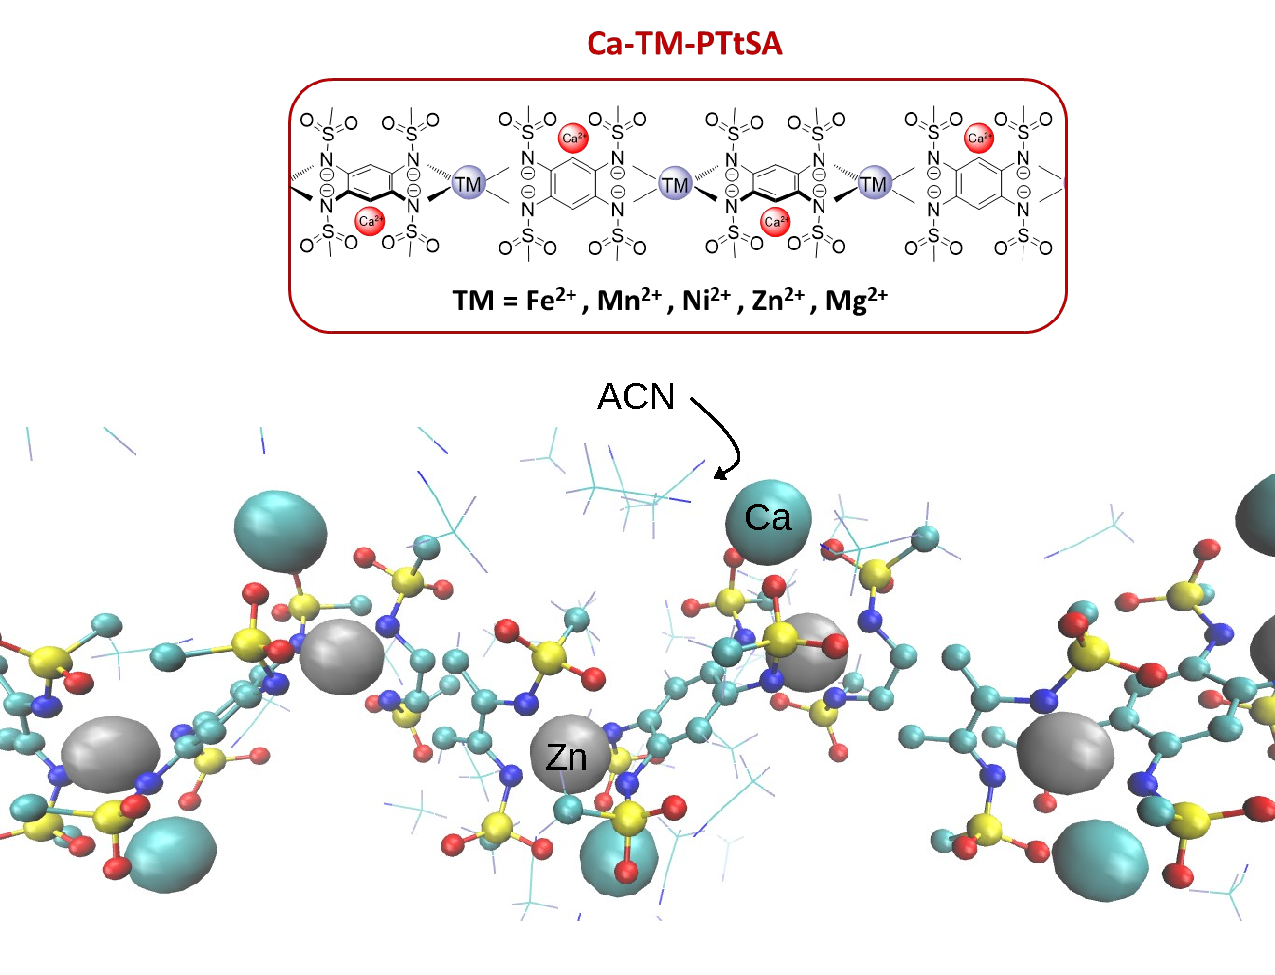
\includegraphics[width=\linewidth]{structure}
	\end{figure}
	
\begin{figure}[!h]
	\centering
	\includegraphics[width=.8\linewidth]{FigureS1}
	\caption{Radial distribution function between the redox cation and the polymer's oxygens, using the last \SI{35}{\pico\second} of the simulation.}
\end{figure}

\begin{figure}[!h]
	\centering
	\includegraphics[width=.8\linewidth]{FigureS2}
	\caption{Radial distribution function between the redox cation and the solvent, using the last \SI{35}{\pico\second} of the simulation.}
\end{figure}

\begin{figure}[!h]
	\centering
\includegraphics[width=.8\linewidth]{FigureS3}
\caption{Radial distribution function between the binding cation (Zn) and the polymer's nitrogens, using the last \SI{35}{\pico\second} of the simulation.}
\end{figure}

\begin{figure}[!h]
\centering
\includegraphics[width=.8\linewidth]{FigureS4}
\caption{Radial distribution function between the binding cation (Zn) and the polymer's oxygens, using the last \SI{35}{\pico\second} of the simulation.}
\end{figure}

\begin{figure}[!h]
\centering
\includegraphics[width=.8\linewidth]{FigureS5a}
\includegraphics[width=.8\linewidth]{FigureS5b}
\caption{Distribution of the interior angles of the zig-zag formed by the polymer,  obtained using the last \SI{35}{\pico\second} of the simulation}
\end{figure}

\begin{figure}[!h]
\centering
\includegraphics[width=.8\linewidth]{FigureS6a}
\includegraphics[width=.8\linewidth]{FigureS6b}
\caption{Distribution of the rolling angle between the sulfonamide units,  obtained using the last \SI{35}{\pico\second} of the simulation}
\end{figure}
	
\end{document}